\chapter{TKE Budget}
\label{ch:tke}

Open from \uipth{3.\ Analysis $\to$ TKE Budget}.

The turbulent kinetic energy $k = \tfrac{1}{2}\langle u'_i u'_i \rangle$ evolves according to the TKE transport equation (Pope, 2000, Ch.\ 5):
\[
\underbrace{\frac{\partial k}{\partial t}}_{\text{unsteady}} + \underbrace{\langle U_j \rangle \frac{\partial k}{\partial x_j}}_{C} = \underbrace{-\langle u'_i u'_j \rangle \frac{\partial \langle U_i \rangle}{\partial x_j}}_{P} \underbrace{- \frac{\partial}{\partial x_j}\!\left(\tfrac{1}{2}\langle u'_i u'_i u'_j \rangle + \frac{\langle p' u'_j \rangle}{\rho}\right)}_{D} - \underbrace{\nu \left\langle \frac{\partial u'_i}{\partial x_j}\frac{\partial u'_i}{\partial x_j} \right\rangle}_{\varepsilon}
\]

Production $P$ represents the rate at which turbulent energy is generated by the interaction of Reynolds stresses with the mean velocity gradients. Convection $C$ describes the transport of $k$ by the mean flow. Turbulent diffusion $D$ redistributes energy in space via triple velocity correlations. Viscous dissipation $\varepsilon$ converts kinetic energy irreversibly into heat at the small scales.

From planar PIV, the dissipation $\varepsilon$ and pressure diffusion cannot be computed directly. \software{uPrime} therefore computes a residual $R = P + D - C$ (for stationary turbulence with $\partial k/\partial t \approx 0$), which absorbs dissipation and any missing out-of-plane contributions. A non-zero $R$ is physically expected and is not an error.

Spatial gradients are computed using central differences with NaN-inpainting near mask boundaries to prevent spurious gradients at wall and shadow edges. Triple correlations for turbulent diffusion are optionally smoothed with a median filter before differentiation to reduce noise amplification.

\begin{notebox}
The residual $R$ absorbs pressure diffusion and viscous dissipation, which cannot be computed from planar PIV. A non-zero residual is expected and is \emph{not} an error in the calculation.
\end{notebox}

\noindent\textbf{Reference:} Pope, S.B. (2000). \textit{Turbulent Flows}. Cambridge University Press.

\begin{table}[htbp]
\centering
\caption{TKE budget terms in \software{uPrime}.}
\begin{tabular}{lll}
\toprule
\textbf{Symbol} & \textbf{Name} & \textbf{Availability} \\
\midrule
$k$                     & Turbulent kinetic energy  & Always \\
$P$                     & Production                & Always \\
$C$                     & Convection                & Always \\
$D$                     & Turbulent diffusion       & Always \\
$R$                     & Residual                  & Always \\
$\partial k/\partial t$ & Unsteady term             & TR data only \\
\bottomrule
\end{tabular}
\end{table}

\section{Using the window}

\begin{stepbox}
\begin{enumerate}[leftmargin=1.5em, topsep=2pt]
  \item Set parameters: enter $U_m$ and $L$ if normalising. Adjust the smoothing kernel if the field is noisy.
  \item Click \uipth{Compute Budget} (only needs to be done once per session).
  \item Select a term from the \uipth{Term} dropdown.
  \item Choose \uipth{2D Contour} or \uipth{Line Profile}.
  \item Click \uipth{Plot}.
\end{enumerate}
\end{stepbox}

In line profile mode the line can be drawn by click-and-drag on the field or set exactly via the $(x_0, y_0)$--$(x_1, y_1)$ coordinate boxes (v0.7.0; see Figure~\ref{fig:coordentry}). TKE $k$ is always overlaid as a dashed reference line regardless of which budget term is selected. Term-visibility checkboxes (\uipth{P}, \uipth{C}, \uipth{D}, \uipth{R}) below the plot control which budget terms appear. All four are checked by default; unchecking one hides it without recomputing.

\begin{figure}[htbp]
  \centering
  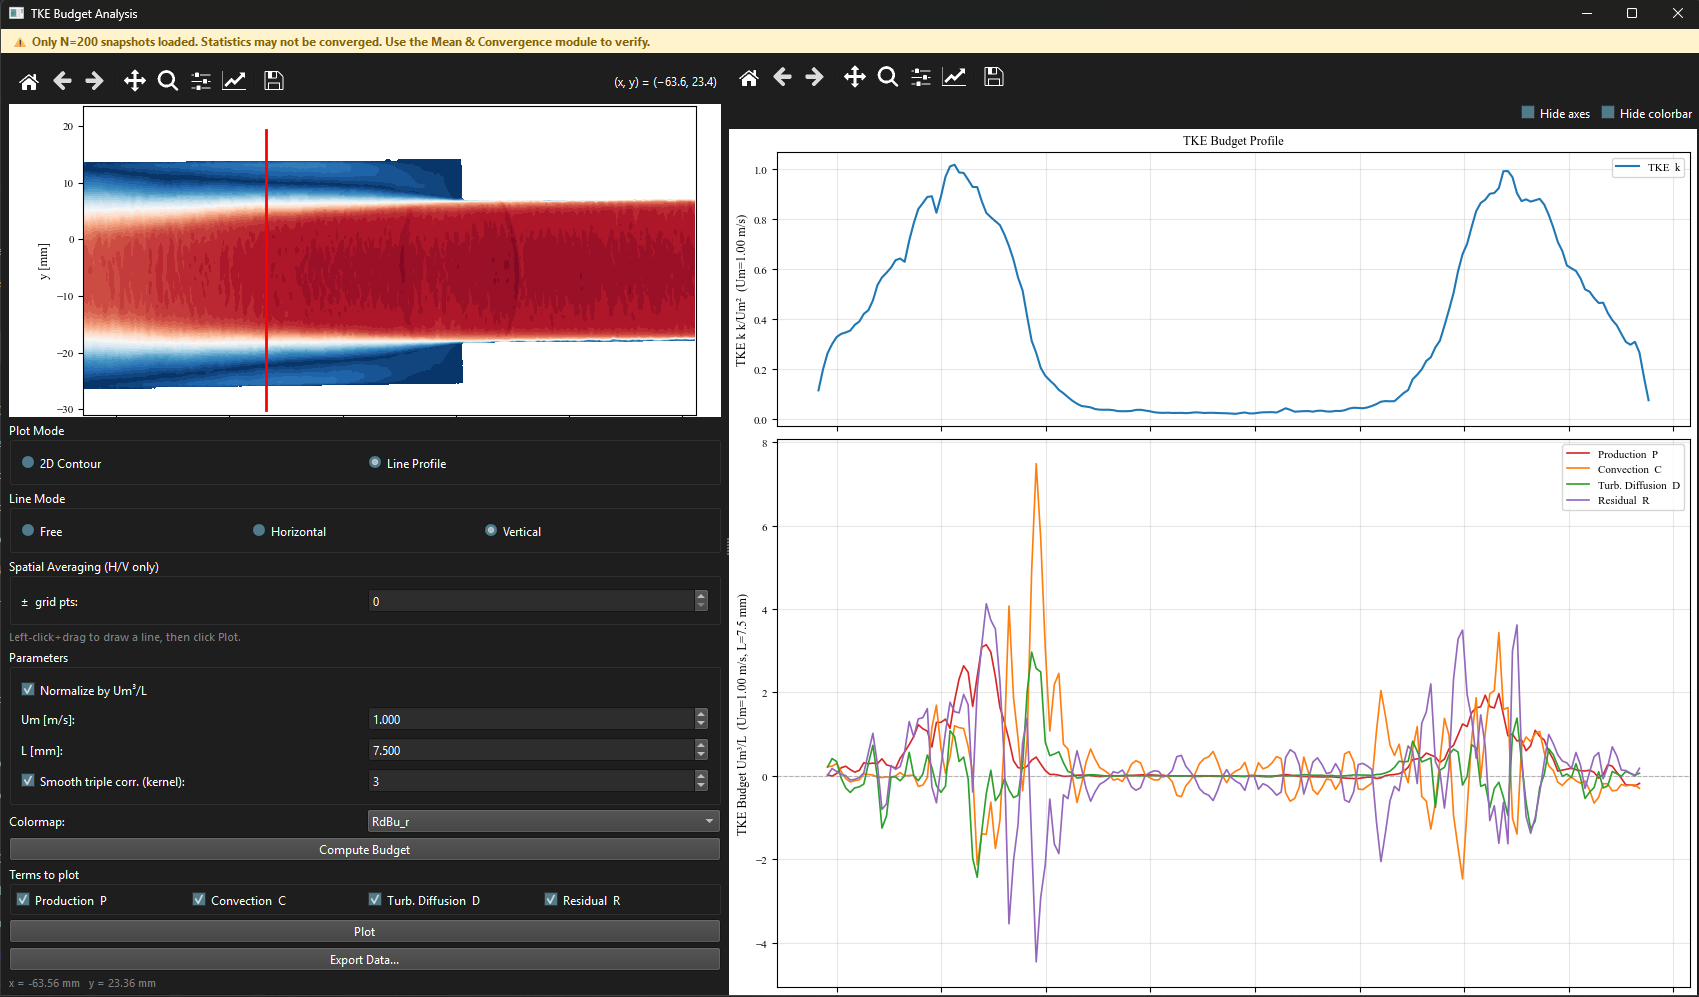
\includegraphics[width=0.92\linewidth]{fig_tke_terms}
  \caption{TKE Budget window in line profile mode showing $P$, $C$, $D$, $R$ along a vertical line through the shear layer. The four checkboxes below the plot control which terms are visible at any time. The mean field reference is shown in the left panel.}
  \label{fig:tkebudget}
\end{figure}

\begin{tipbox}
Enable \uipth{Normalize by $U_m^3/L$} to make the budget terms non-dimensional. TKE $k$ is normalized by $U_m^2$. This is essential when comparing results across different flow conditions or Reynolds numbers.
\end{tipbox}

\section{Multi-case comparison}

The TKE Budget window supports CSV import and overlay (Chapter~\ref{ch:multicase}).

\section{Exporting}

Click \uipth{Export Data\ldots} to save all budget terms together in a single file.

% ============================= CHAPTER 7 ==============================
